
\documentclass[review]{elsarticle}
\usepackage{color}
\usepackage{lineno,hyperref}
\modulolinenumbers[5]

\journal{Nuclear Instruments and Methods B}

%%%%%%%%%%%%%%%%%%%%%%%
%% Elsevier bibliography styles
%%%%%%%%%%%%%%%%%%%%%%%
%% To change the style, put a % in front of the second line of the current style and
%% remove the % from the second line of the style you would like to use.
%%%%%%%%%%%%%%%%%%%%%%%

%% Numbered
%\bibliographystyle{model1-num-names}

%% Numbered without titles
%\bibliographystyle{model1a-num-names}

%% Harvard
%\bibliographystyle{model2-names.bst}\biboptions{authoryear}

%% Vancouver numbered
%\usepackage{numcompress}\bibliographystyle{model3-num-names}

%% Vancouver name/year
%\usepackage{numcompress}\bibliographystyle{model4-names}\biboptions{authoryear}

%% APA style
%\bibliographystyle{model5-names}\biboptions{authoryear}

%% AMA style
%\usepackage{numcompress}\bibliographystyle{model6-num-names}

%% `Elsevier LaTeX' style
\bibliographystyle{elsarticle-num}
%%%%%%%%%%%%%%%%%%%%%%%

\begin{document}

\begin{frontmatter}

\title{Liquid scintillator tiles for high radiation environments }


%% or include affiliations in footnotes:
\author[umd]{Alberto Belloni\corref{mycorrespondingauthor}}
\cortext[mycorrespondingauthor]{Corresponding author}
\ead{abelloni@umd.edu}
\author[umd]{Mahnegar Amouzegar}
\author[iowa]{Burak Bilki}
\author[umd]{Jeff Calderon}
\author[rochester]{Pawel De Barbaro}
\author[umd]{Sarah C. Eno}
\author[baylor]{Kenichi Hatakeyama}
\author[fnal]{James Hirschauer}
\author[umd]{Geng-Yuan Jeng}
\author[baylor]{Joseph Pastika}
\author[fnal]{Kevin Pedro}
\author[umd]{Joshua Samuel}
\author[elmer]{Elmer Sharp}
\author[umd]{Young Ho Shin}
\author[baylor]{Emrah Tiras}
\author[rochester]{Dmitry Vishnevskiy}
\author[umd]{Zishuo Yang}
\author[umd]{Yao Yao}
\author[korea]{Sung Woo Youn}




\address[umd]{Dept. Physics, U. Maryland, College Park MD 30742 USA}
\address[korea]{Institute for Basic Science, Center for Axion and Precision Physics Research, IBS Center for Axion and Precision Physics Research
Room 4315, Department of Physics, Natural Science Building (E6-2), KAIST,
291 Daehak-ro, Yuseong-gu, Daejeon 305-701, South Korea}
\address[elmer]{Elmer Sharp Engineering, 7007 Leesville Blvd. Springfield, VA 22151}
\address[fnal]{Fermi National Accelerator Laboratory, Batavia, IL, USA}
\address[baylor]{Baylor University, Waco, Texas, USA}
\address[iowa]{The University of Iowa, Iowa City, IA, USA}
\address[rochester]{The University of Rochester, Rochester, NY, USA}

\begin{abstract}
Future experiments in high energy and nuclear physics may require
large, inexpensive calorimeters that can continue to
operate after receiving doses of 50~Mrad
or more. We present the results of a study of a scintillator tile
based on EJ-309 liquid scintillator using cosmic rays, test beam, and
${\rm ^{60}Co}$ irradiations that shows little degradation of light output
under irradiation.
\end{abstract}

\begin{keyword}
organic scintillator\sep liquid scintillator\sep radiation
hardness \sep calorimetry
\end{keyword}

\end{frontmatter}

\linenumbers

\section{Introduction}
Sampling calorimeters using plastic scintillator tiles with
wavelength-shifting (WLS) fibers as their active element, such as the CDF plug
calorimeter~\cite{Aota1995557} and the CMS Barrel~\cite{CMSHB} and
Endcap~\cite{HCALTDR1997} hadron calorimeters, are popular due to their
low cost and ease of construction. Plastic scintillator is available
commercially from companies such as St. Gobain and Eljen Technology. When
irradiated, however, the performance of plastic scintillator and WLS
fibers deteriorates; light self-absorption (yellowing) increases and
light output decreases. The resulting loss of light output for this
kind of tile has been studied using irradiations
from electron linacs and ${\rm ^{60}Co}$ sources~\cite{vasken,ByonWagner1993263}.
Generally, the light output decreases exponentially with dose, with an
decay constant on the order of a few~ Mrad. Future high energy and nuclear
experiments, however, may have to operate in environments that will
deliver doses of tens of Mrad.
Previous studies of liquid scintillator have shown little decrease
of light output with dose ~\cite{zornliquid,Klein1967399,berlman}.
In this paper, we present the design
and optimization of a liquid scintillator tile
that can operate in this kind of environment.
An earlier liquid tile design is described in~\cite{liquidrandy}.

\section{Tile design}
\label{sec:design}
Our tile is based on EJ-309 scintillator, from Eljen Technology, which
uses naphthalene as the substrate with wavelength shifting additives.
EJ-309 has a light output that is 75\% of anthracene, a wavelength of
maximum emission of 424~nm, a refractive index of 1.57, and a flash
point of $\rm{144^o}$\,C. The high flash point is important for its
suitability for a collider environment.

The design of a tile to hold the liquid needs to consider light
collection efficiency, light collection uniformity, and cost. The
container should not leak, and there should not be interactions
between the container and its contents that degrade the light output
over time or compromise the integrity of the
container. 
Figure~\ref{fig:tiledesign} shows the mechanical
construction of our prototype. The case is made of aluminum. Two
transparent quartz support tubes
run through the
liquid and can hold either a WLS fiber or liquid
wavelength shifter.
When a WLS fiber was
used, the end of the fiber not connected to the photodetector was
coated with Al to increase the light output unless otherwise
noted. The support tube is sealed to the case with a Viton
fluoroelastomer o-ring. The thicknesses of the top and bottom Aluminum
plates are 0.5\,mm. The total internal volume is 88\,mm x 88\,mm x
4\,mm. The inner surface of the container is a lapped and polished
Al-6061 available from McMaster Carr. The material comes with a
plastic coating that can be used to maintain its mirror quality during
the machining process and then is removed before the welding step. The
liquid was transferred into the container in an inert atmosphere, as
contamination with Oxygen decreases the light output.

Several variations on this design were constructed. For the default
design, the thickness of the liquid is 4\,mm. A version with a 6\,mm
thickness was also made. The default
support tubes, from Atlantic International, were quartz with an inner
diameter of 1.3\,mm and were used with Kuraray Y-11 fiber (doping of
200~ppm), double-clad.
The index of refraction was measured at the Quattrone
Nanofabrication Facility at the University of Pennsylvania to be
1.653.
As an alternative, two types of
Quartz tubes filled with liquid wavelength
shifter (capillaries) were also used.  
One set, of ordinary quartz, had an outer diameter of 2\,mm,
an inner diameter of 1\,mm, and a measured index of refraction of 1.548.
Another used special radiation-resistant quartz and had an outer diameter of 1\,mm and an
inner diameter of 0.4\,mm.  Its index was not measured.
The liquid wavelength shifter was a prototype
material from Eljen, and is not yet a commercial item. The liquid
wavelength shifter has an emission maximum from between 481 and 492\,nm
and a decay time between 2 and 8~ns. The solvent was the same as that
used for EJ-309. Sapphire tubes, with an index of 1.653,
were also tested with both liquid and
plastic wavelength shifter.


\begin{figure}[!ht]
\begin{center}
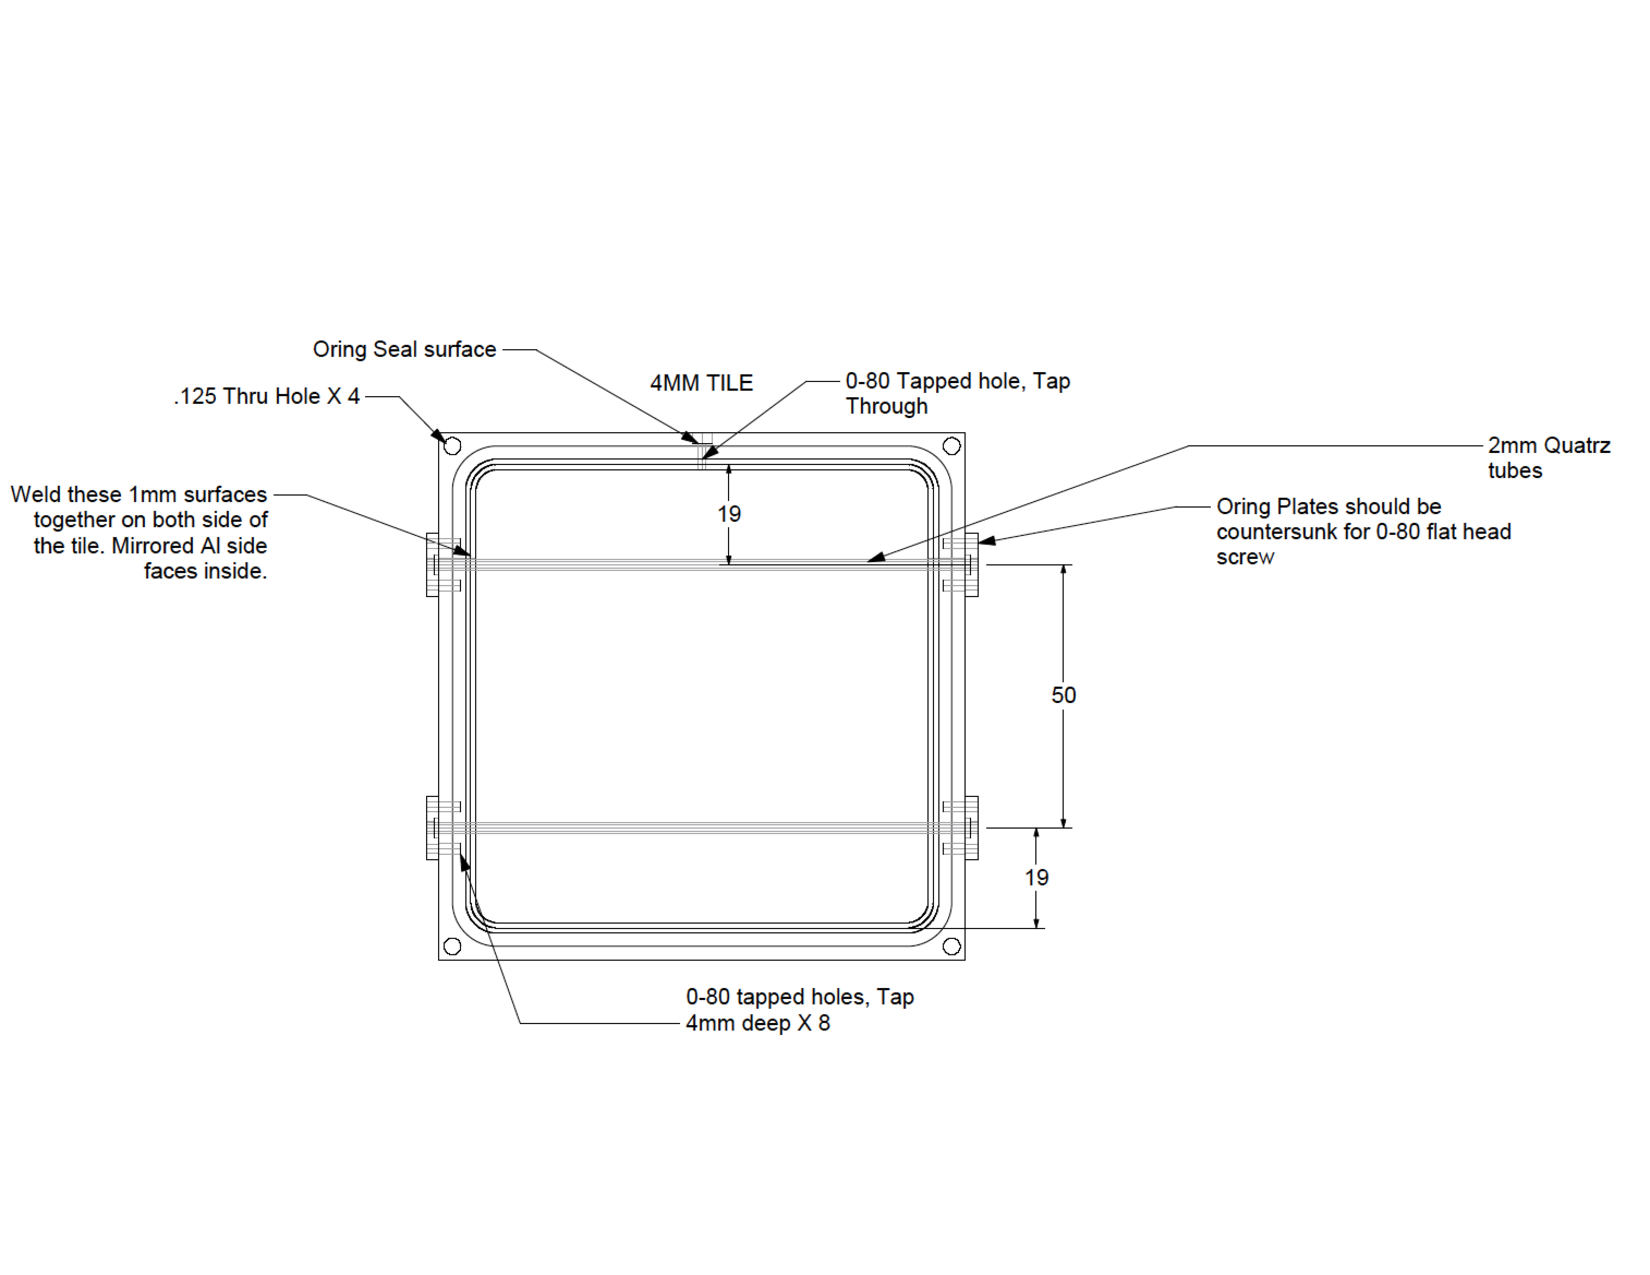
\includegraphics[width=0.95\textwidth]{./figures/mechanicaldesign.pdf}
\caption{Mechanical design of a liquid scintillator tile. Units are
  [mm].}
\label{fig:tiledesign}
\end{center}
\end{figure}

In what follows, the results shown are for the mirrored tile with 4\,mm
thickness, ordinary quartz support tubes, and a 0.9\,mm diameter Y-11 WLS fiber,
unless otherwise stated.

\section{Light yield and uniformity as measured in test beam}

The light yield and uniformity of the tiles was measured in the H2
test beam facility at CERN using 120\,GeV muons. The trigger required
coincidence of two out of four plastic scintillator hodoscopes. The
effective beam cross sectional area, after trigger requirements, was
14x14\,cm$^2$. The positions of the muons were measured with four
wire chambers. The position obtained from the counter closest to the
prototype was used. We also required the signal in each wire chamber
be consistent with that of a single muon, and that the difference in
positions in sequential chambers be consistent within uncertainties.
As many groups were using the same test beam, there was material
upstream of our counters. For some runs, several steel blocks were
used to support experiments upstream of our counters. Because the
muons were high energy, the probability of a muon-induced shower was
non-negligible. (This was verified later at a test beam at FNAL that
had a cleaner beam line, by varying the material in front of the tile
and through simulations with varying amounts of material.) We present here the
results from the runs and tiles with the smallest upstream material.

The WLS fiber was connected to a clear fiber using a
connector designed at FNAL. The clear fiber was lead away from the
beam line. The light output was measured using a Hamamatsu
R7600U-200-M4 photomultiplier tube and a custom ASIC that integrates
and digitizes the resulting charge, called the ``QIE''~\cite{qie}.
The photomultiplier has a peak quantum efficiency of 40\% at a
wavelength of 400\,nm and produces a clear single photoelectron (pe)
peak. The integrated charge is digitized every 25\,ns. Ten
digitizations were recorded per muon trigger. The sum of the signal
in the ${\rm 4^{th}}$ to ${\rm 7^{th}}$ sample was used.

The average number of pe's produced per minimum ionizing particle
(mip) was estimated by doing a Gaussian fit to the peak centered on
the pedestal. The mean number of pe's was calculated using the
fraction of events in this peak, assuming a Poisson distribution. The
nominal tile produced 1.7\,pe's per mip.
%Tiles for the CMS hadron
%calorimeter typically produce 3\,pe's per mip~\cite{CMSHB}.
A plastic tile (SCSN-81 with Y-11 fiber) with dimensions 10\,cm x 10\,cm x 4\,mm tested
at the same time gave 1.8 pe/MIP.
The results
have a systematic uncertainty related to the handling of the events
with showering muons. We evaluate this uncertainty by looking at the
results after truncating the distribution at around 25\,pe's (2000 adc
counts). The results were stable to within 5\%. In addition, runs
taken with varying amounts of material in front of our detector
(up to 20\,cm of steel)
resulted in a 15\% variation in light yield.
We therefore take a 16\% uncertainty due to upstream material.

The uniformity of the light collection was also studied at the CERN
test beam. Figure~\ref{fig:fig1} shows the fraction of events with at
least 1\,pe versus the impact position of the mip along the axis
parallel to the support tubes (left) and perpendicular to the support
tubes (right). As expected, there is little dependence on the
coordinate parallel to the support tubes. The light yield does depend
on the perpendicular distance. The light collection efficiency is
maximum for muons near the WLS fiber and is approximately 20\%
lower for muons in the center or edges of the tile. For most hadron
calorimetry applications, we verified through simulation that this
degree of non-uniformity would not adversely affect jet resolutions.

\begin{figure}[h]
\centering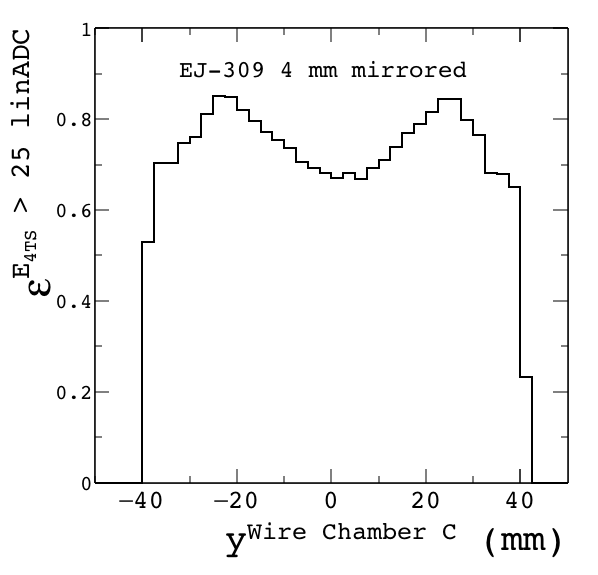
\includegraphics[scale=0.5]{./figures/fiducial3.png}
\centering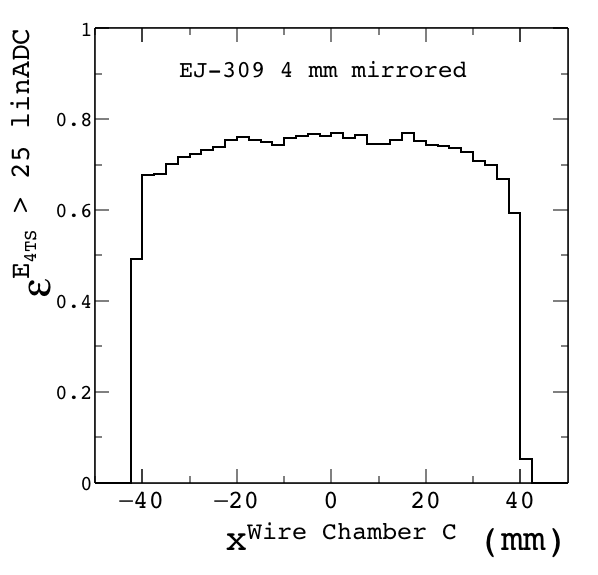
\includegraphics[scale=0.5]{./figures/fiducial2.png}
\caption{For the nominal liquid tile, fraction of mips with at least
  one pe as a function of the impact position of the mip along the
  axis parallel to the support tubes (left) and perpendicular to the
  support tubes (right).{\color{red} Geng Yuan will remake to publication quality}}
\label{fig:fig1}
\end{figure}

\section{Light yield dependence on tile parameters}

The dependence of the light yield on variations in the design
parameters was studied using cosmic ray data taken at the University
of Maryland. Scintillator-based counters above and below the tile
were used for triggers. The tile light output was measured using a
Hamamatsu R7600U-200-M4 photomultiplier tube. Fibers were connected
to the tube using optical glue. Data was collected with a Tektronix
MSO 5204 oscilloscope. No attempt was made to select minimum ionizing
muons. The muons thus are low energy and will produce more light than
those studied at the CERN test beam.

We found an average of 
$2.88\pm 0.05$\,pe for the nominal tile. A similar tile but without
the mirroring yielded $1.98\pm 0.03$\,pe, a reduction of a factor of
1.45. A tile with a 6\,mm thickness of liquid, non-mirrored, yielded
$2.61\pm 0.05$\,pe, an increase over the 4\,mm non-mirrored tile of a
factor of 1.32.
Figure~\ref{fig:thickness_comp} shows the collected charge (arbitrary units)
for the three different configurations.

\begin{figure}[!ht]
\begin{center}
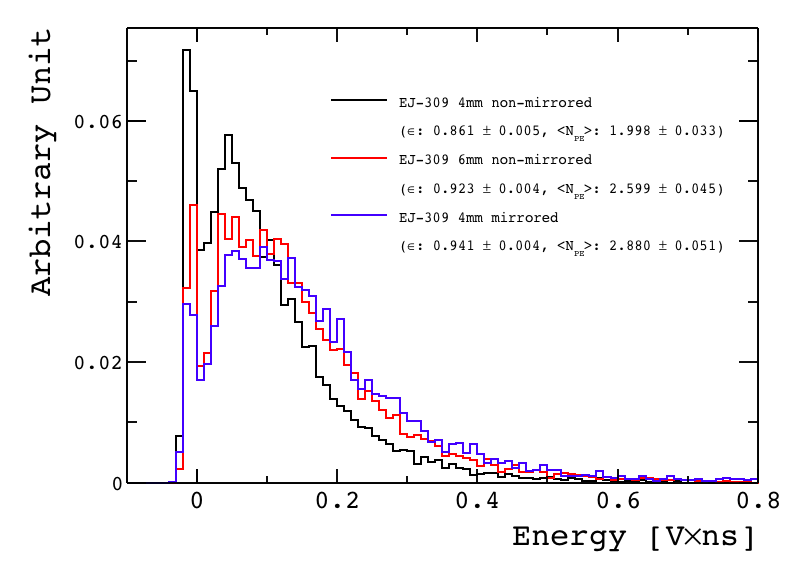
\includegraphics[width=0.8\textwidth]{./figures/list_NEW_PROTOTYPES_all.png}
\caption{Comparison between the light output (arbitrary units)
  of liquid scintillator
  tiles with different thickness and different treatment of the
  aluminum surface in contact with the liquid scintillator. The light
  is readout with the same 0.9\,mm-thick Y11 plastic WLS fiber. The
  three distributions are normalized to have the same number of events
  in the pedestal.{\color{red} Geng Yuan will remake to publication quality.  I hate the normalization of these plots.  can we normalize to number of muons?  also, what is mpv?   needs to be clear}}
\label{fig:thickness_comp}
\end{center}
\end{figure}


The light yield was also studied using a capillary, filled
with liquid WLS, instead of a quartz tube containing plastic WLS, since
plastic WLS is susceptible to radiation damage.
The capture efficiency of the WLS for the two different configurations
depends crucially on the index of the surrounding media.  For the WLS fiber,
there is an air gap with an index of 1.  For the capillary, the liquid WLS
is instead bordered by quartz, with an index of {\color{red} jeff's number}.
The plastic and liquid WLS have very similar
indices of refraction (1.57).  In both cases, the shifted light propagates
in the WLS, but the capture efficiency is higher for the lower index air.
Figure~\ref{fig:y11_vs_cap} shows the charge collected (in arbitrary units)
from cosmic muons for the two different configurations.  The fraction of
events in the pedestal, which is the Gaussian-shaped peak at low charge,
can be used to calculate the fraction of muons producing at least one pe
(light collection efficiency)
and the mean number of pe's per muon.
The light collection efficiency
is  $92\%$ for the plastic WLS and  $45\%$ for the liquid.  The light
yield for the liquid is half that of the plastic.
The light collection efficiency with the liquid could be improved
if lower index quartz
could be found.

\begin{figure}[!ht]
\begin{center}
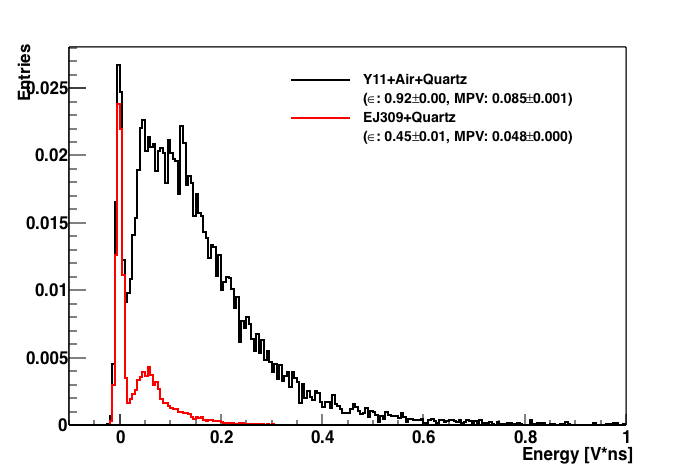
\includegraphics[width=0.8\textwidth]{./figures/list_RO_FIBER_all_norm.png}
\caption{Comparison between the light output of a liquid scintillator
  tile equipped with a plastic WLS fiber, and a capillary filled with
  liquid WLS. The two distributions are normalized to have the same
  number of events in the pedestal.{\color{red} Geng Yuan will remake to publication quality, and will make a more sensible normalization since i hate this normalization to the pedestal.  why not normalize to the same number of muons?}}
\label{fig:y11_vs_cap}
\end{center}
\end{figure}




Finally, we tested the performance of the same tile, 4\,mm-thick, with a
mirrored aluminum surface, as a function of the thickness of the
readout plastic WLS fiber. We tested three plastic fibers, with a
thickness of 0.5\,mm, 0.9\,mm, and 1\,mm. We measured that the higher the
fiber thickness, the higher the efficiency and light output, as shown
in Figure~\ref{fig:fiber_thickness_comp}.
{\Large \color{red} This would be much more useful as a plot of pes versus fiber thickness.  If we can not get this, I say remove it.}

\begin{figure}[!ht]
\begin{center}
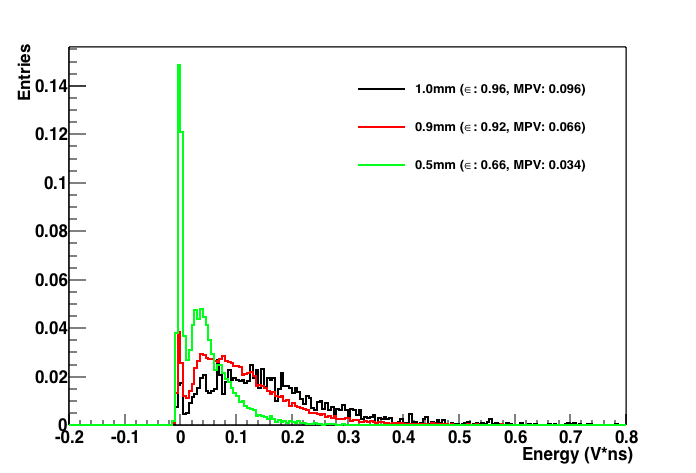
\includegraphics[width=0.8\textwidth]{./figures/list_Fiber_Thickness_all_1.png}
\caption{Comparison between the light output of liquid scintillator
  tiles readout with plastic WLS fibers with different thickness. The
  three distributions are normalized to have the same number of
  events.{\color{red} Geng Yuan will remake to publication quality}}
\label{fig:fiber_thickness_comp}
\end{center}
\end{figure}

\section{Radiation hardness tests}

Several different tests were made using irradiations with a
$\rm{^{60}Co}$ source at the University of Maryland.
Performance of the tile under irradiation in a proton-proton collision
environment will be the subject of a future paper.

A dark-glass vial containing 125\,ml
of liquid scintillator was irradiated with $\gamma$-rays to a
dose of 50\,Mrad, at a dose rate of 1\,Mrad/hr.
Figure~\ref{fig:ej309_irradiated} compares the integrated charge (arbitrary units)
from the same tile when filled with unirradiated liquid and irradiated liquid.
The efficiency and light output from the two measurements are
consistent within the uncertainty, indicating that EJ-309 is
radiation-tolerant to $\gamma$-ray irradiations.

\begin{figure}[!ht]
\begin{center}
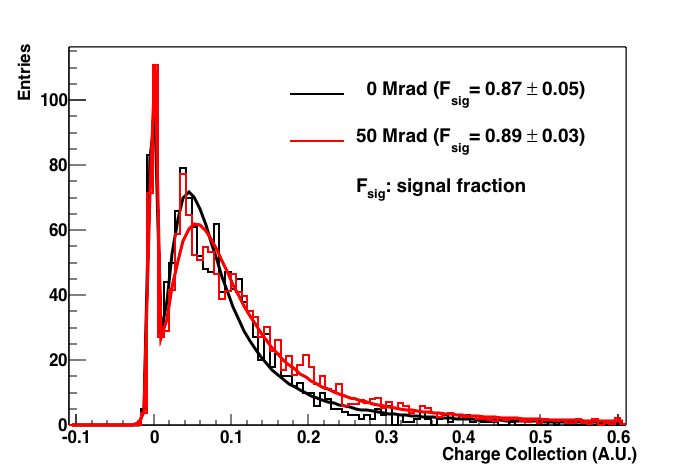
\includegraphics[width=0.8\textwidth]{./figures/RD_R7600_1_0_DBF_ALM_GRS_TH450_100814_all_1.png}
\caption{Comparison between the light output of a liquid scintillator
  tile filled with unirradiated (black) and irradiated (red) liquid
  scintillator. The two distributions are normalized to have the same
  number of events in the pedestal.{\color{red} Geng Yuan will remake to publication quality}}
\label{fig:ej309_irradiated}
\end{center}
\end{figure}

{\Large\color{red} I want to try irradiating an entire tile with the rad hard 1mm tubes from Randy and put the results here as well.}

\section{Comparison with simulation, and optimization}
We use the GEANT4~\cite{Agostinelli2003250} package to simulate the
optics of our tile. GEANT4's optical package includes simulations of
refraction, reflection, wave length shifting, and light attenuation.
A variety of options for the reflection are available. We used the
``Specular Spike'' option for the Al and an absorption length of 2\,m for
the EJ-309. When simulating the WLS fiber, an air gap was included
between the fiber cladding and the support tube, while no such gap
exists for the simulation of the capillary. An index of refraction of
1.57 is used for the EJ-309. The index for sapphire used was 1.77.
For quartz, values between 1.46 and 1.55 were used. Photons are
generated at random positions inside the liquid volume, with a
spectrum corresponding to the emission spectrum of EJ-309.

As shown in Figure~\ref{fig:simeff} left, we find the simulation
reproduces the light collection non-uniformity when a reflectivity of
0.9 is used for the mirrored Al.

\begin{figure}[!ht]
\begin{center}
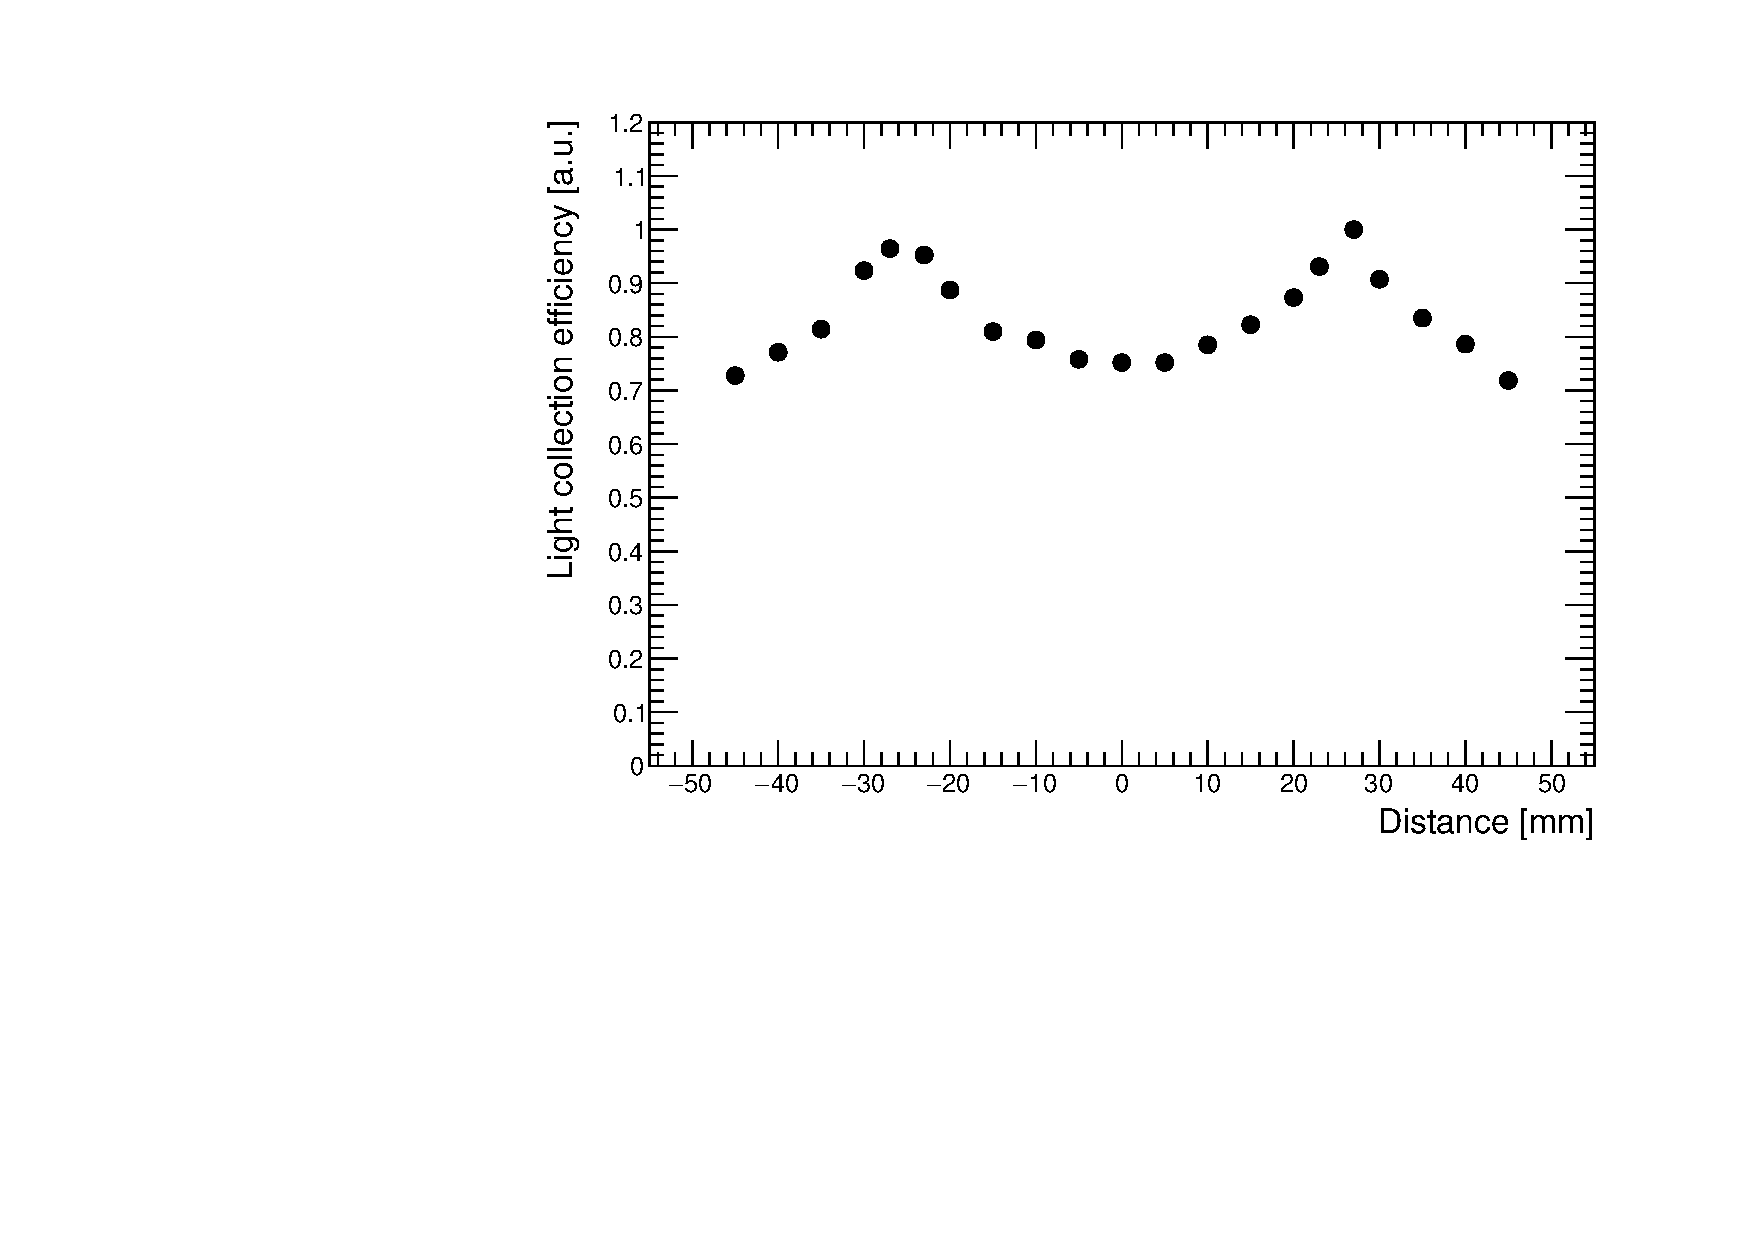
\includegraphics[width=0.8\textwidth]{./figures/geant_uniformity_plot.pdf}
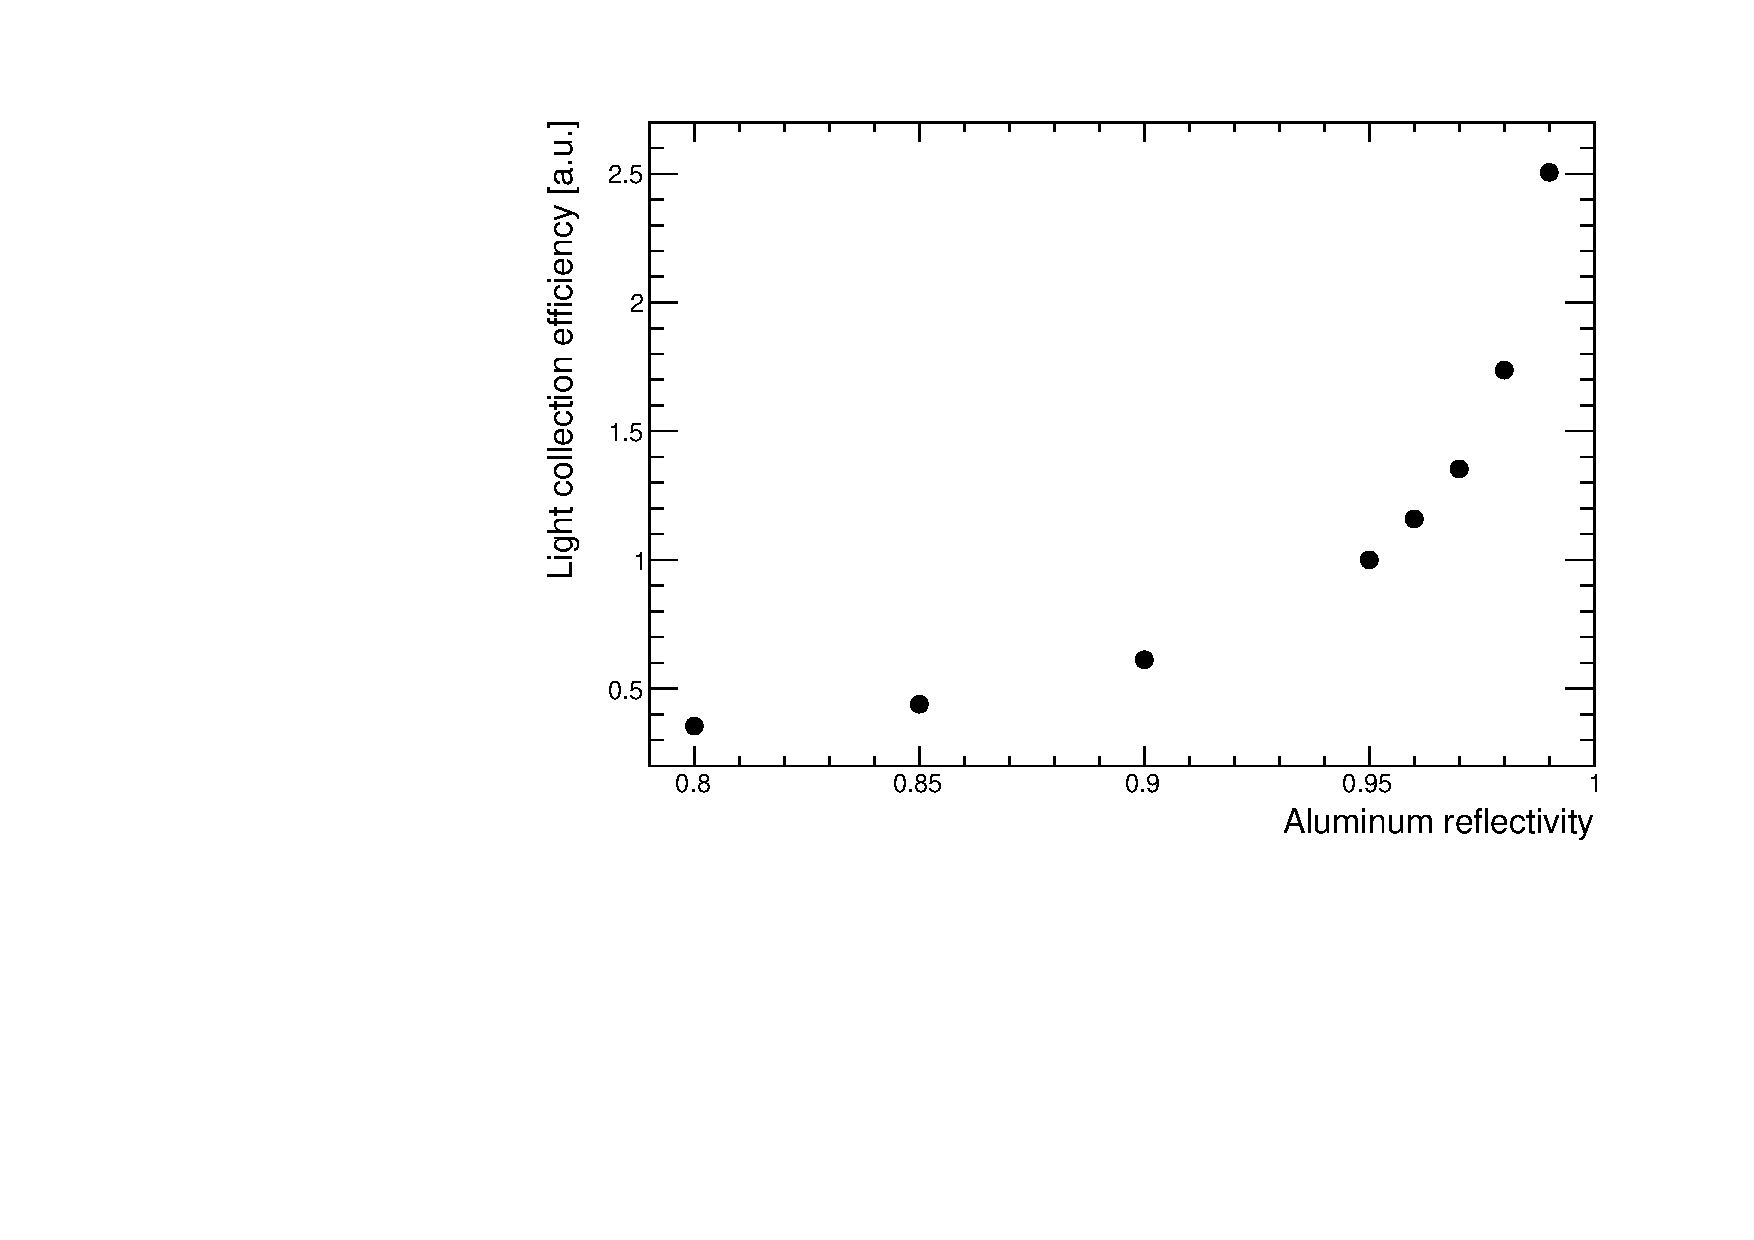
\includegraphics[width=0.8\textwidth]{./figures/geant_reflectivity_plot.pdf}
\caption{(left) Ratio of light yield to maximum light yield from
  simulated tile as a function of the distance perpendicular to the
  support tubes, normalized to the efficiency at the position of the support tubes.
    (right) Light collection efficiency vs Aluminum
  reflectivity, normalized to a reflectivity of 0.95.
  }
\label{fig:simeff}
\end{center}
\end{figure}

We find that the light collection efficiency is a strong function of
the reflectivity of the Al (Figure~\ref{fig:simeff} right).

We find the best light collection comes when the support tube has the
lowest possible index of refraction for liquid WLS. The opposite is
true for a fiber with an air gap (and plastic WLS). For a 1\,mm
diameter for the WLS, the light collection efficiency increases by a
factor of 3.57 going from an
index of 1.55 to 1.46 for liquids. Presumably this difference would
decrease as the reflectivity of the Al increases. For a fiber with an
air gap, the efficiency decreases by a factor of 1.42 going from an index of 1.77 to 1.46.

\section{Conclusions}

We presented results for a liquid scintillating tile using WLS fiber readout. For our nominal design, $1.7\pm 0.2$\,pe's
were produced for minimum ionizing particles.

\section{Acknowledgments}
The authors would like to thank Randy Ruchti of Notre Dame for
providing the capillaries and both Randy and Chuck Hulbut of Eljen
Technologies for
advice in general on liquids.
Yasar Onel's group at the University of
Iowa for help with the test beam. We would like to thank Eric
Johnston from the Quattrone Nanofabrication Facility at the University
of Pennsylvania for measuring the indices of refraction of our support
tubes. 
The authors would like to thank {\color{red} various people} at
the University of Maryland's Nuclear Reactor and Radiation
Facilities group for assistance
with the irradiations.
 We would like to thank the University of Maryland
FabLab, especially {\color{red} who helped}, for help with fiber sputtering.
This work was supported in part by U.S. Department of Energy
Grant DESC0010072.

\section*{References}

\bibliography{aliquidtile}

\end{document}
